\documentclass[11pt]{article}
\usepackage{geometry}
% Math packages.
\usepackage{amsmath,amssymb,amstext,amsfonts}
% Add figures.
\usepackage{graphicx}

% Metadata
\author{Jarod Klion}
\title{Solution Report for Assignment 1}

\newcommand{\norm}[1]{\lVert#1\rVert}
\newcommand{\abs}[1]{\lvert#1\rvert}

\begin{document}

\maketitle

\section{Executive Summary}

In this report, we consider translation, rounding, and addition in the floating point system $\mathcal{F}(t, 10, e_{min}, e_{max})$ using either chopping or round-to-nearest strategies. The errors of our routines are validated empirically through the means, variances, and histograms obtained from running a large number of experiments. Results are obtained and discussed for the randomly generated data within the given exponent bounds, $e_{min} = -9$ and $e_{max} = 0$, and $t = 5$.

\section{Statement of the Problem}

The computational approximations of decimal numbers, floating point numbers, are essential to the mathematical operations found in nearly all computing applications. The proximity of this representation to the actual decimal number itself is used to determine the accuracy of given floating-point routines. We analyze the accuracy of our translation, rounding, and addition routines in our floating-point system using the correctness test for translation and addition, the accumulation bound, and conditioning analysis, respectively:
\begin{enumerate}
	\item $\abs{\frac{fl(x) - x}{x}} = \abs{\delta} \leq u_n$
	\item $ \frac{\abs{(f_1 + f_2) - (f_1 \boxplus f_2)}}{\abs{f_1 + f_2}} = \abs{\delta} \leq u_n$
	\item $\abs{\hat{s}_n - s_n} \leq \sum \norm{\xi_{1:n}}_1 u_n = (n-1)\norm{\xi_{1:n}}_1 u_n$
	\item $\kappa_{rel} \approx \max\limits_{p_{1:n}} c_{rel}^{p_{1:n}}$, where $c_{rel}^{p_{1:n}} = \frac{\abs{\sum_{i=1}^{n} x_i - \sum_{i=1}^{n} (x_i + p_i)}}{\abs{\sum_{i=1}^{n} x_i}}\frac{\norm{x_{1:n}}_1}{\norm{p_{1:n}}_1}$
\end{enumerate}

\section{Description of the Algorithms and Implementation}

The previously mentioned routines for translating, rounding, and adding floating point numbers, as well as their respective error checks above, are translated directly into respective functions in \textbf{Python}. The float translation function takes three arguments: (1) a real number, $x$, (2) the number of digits to store, $t$, and (3) a flag, \emph{RoundtoNearest}. The round-to-nearest function accepts four integer arguments: (1) the remainder, (2) mantissa, $m$, (3) exponent, $e$, and (4) the number of digits to store, $t$. The float addition function accepts four arguments: (1) a translated float, $x$, (2) a translated float, $y$, (3) the number of digits to store, $t$, and (4) a flag, \emph{RoundtoNearest}. The accumulation function accepts one argument: (1) an array of floats, $x$, and calculates their sum. Each error check takes in their respective arguments as shown in the expressions above.

\section{Description of the Experimental Design and Results}

For each algorithm, the error bounds are directly calculated for each run with the mean value and variance of all runs taken at the end to validate the statement. The results of all the runs are also plotted on a histogram to verify visually that all obtained values fall within the respective bound. Considering every test has an upper bound given by $u_n = \frac{10^{-4}}{2}$ in this assignment, we must verify that all tests yield $\delta$ that are either equal to or less than that given value.  

In figure \ref{fig:translate}, we can see that all achieved error values for our translation routine are less than $u_n = 5 \times 10^{-5}$, meaning they fall within the bound. We can also see from the histogram that there are no real outliers as with enough experiments ran, each possible error value occurs relatively equally. A similar pattern follows for our addition routine, which can be seen in figure \ref{fig:correctness}.

In the left part of figure \ref{fig:accumulation}, we see a histogram of the relative error between the actual sum of the numbers and the floating point sum. On the right part of figure \ref{fig:accumulation}, we see that the error for this accumulation routine appears to be a normal distribution with mean $0.25$. Looking at both of these histograms together to compare values, we see that the differences between the sums tend extremely close to 0 with the majority being $1 \times 10^{-14}$ which is less than any of the error values achieved, validating the bound.

Lastly, in figure \ref{fig:condition}, we see that the relative error between two exact sums is typically quite close to one, with most obtained results being within $0.01$ of this value. This is consistent with the approximated condition number, which was about equal to one as well.

\section{Conclusions}

Our results illustrate that, for our floating point system $\mathcal{F}(5, 10, -9, 0)$, the implemented translation, rounding, and addition routines satisfy all error bounds. A topic not considered in this report is how to handle overflow or underflow detection for our given float translations. In many circumstances, the randomly generated samples were assumed to be within bounds, and the lack of outliers makes us confident that they were; however, the lack of explicit detection means some of the calculated means could have been affected by outliers in the data. A floating-point system where this detection is in-place could be studied further in the future or possibly found in current literature.


\section{Figures}
\begin{figure}[h!]
	\centering
	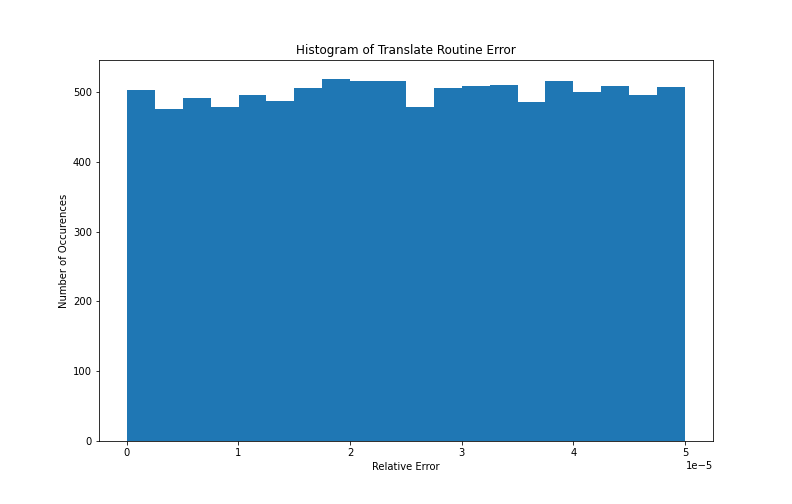
\includegraphics[width=\linewidth]{../figures/Translation Histogram}
	\caption{Error results for the translate to float routine}
	\label{fig:translate}
\end{figure}

\begin{figure}[h!]
	\centering
	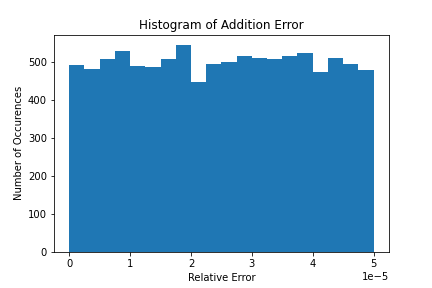
\includegraphics[width=0.8\linewidth]{../figures/Correctness Histogram}
	\caption{Relative error bound for $\boxplus$ for round-to-nearest}
	\label{fig:correctness}
\end{figure}

\begin{figure}[h!]
	\centering
	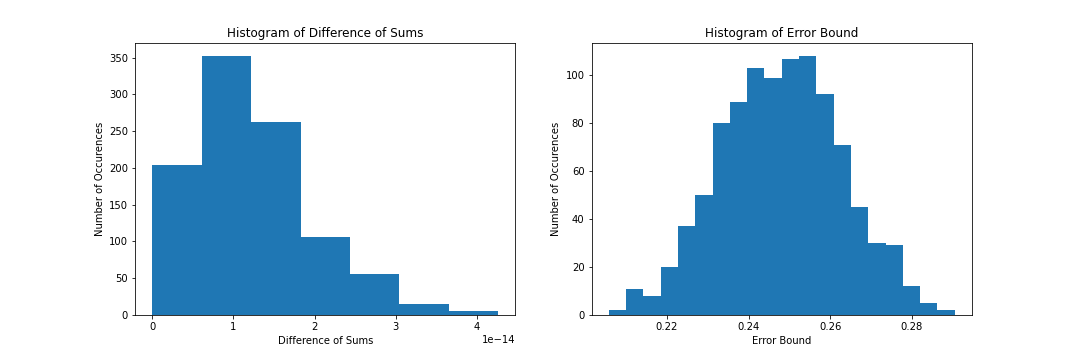
\includegraphics[width=1.2\linewidth]{../figures/Accumulation Histogram}
	\caption{Left: Error between the float sum and regular sum. Right: Error bound for accumulation for round-to-nearest.}
	\label{fig:accumulation}
\end{figure}

\begin{figure}[h!]
	\centering
	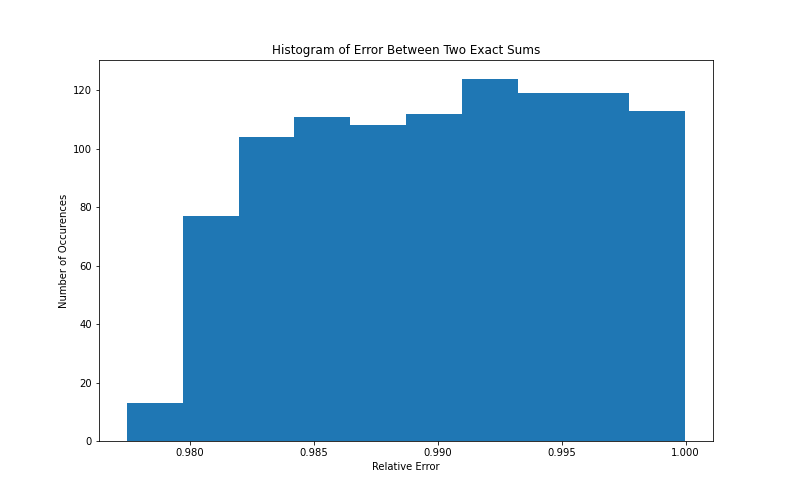
\includegraphics[width=\linewidth]{../figures/Condition Number Histogram}
	\caption{Relative error between two exact sums of a set of real numbers used to validate the approximated condition number.}
	\label{fig:condition}
\end{figure}

\end{document}
